%------------------------------------------------------------
\documentclass[conference,letterpaper]{IEEEtran}
\usepackage[spanish]{babel}
\usepackage[utf8]{inputenc}
\usepackage{amsmath}
\usepackage{amssymb}
\usepackage[usenames]{color}
\usepackage[pdftex]{graphicx}
\usepackage{tcolorbox}
\usepackage[colorlinks, linkcolor=black]{hyperref}
\tcbuselibrary{listingsutf8}
%------------------------------------------------------------
\graphicspath{{../pdf/}{../jpeg/}}
\DeclareGraphicsExtensions{.pdf,.jpeg,.png}
%------------------------------------------------------------
\hyphenation{op-tical net-works semi-conduc-tor}
%------------------------------------------------------------
\definecolor{Fucsia}{RGB}{193,124,250}
\definecolor{Azul}{RGB}{20,80,200}
%------------------------------------------------------------
\DeclareRobustCommand*{\IEEEauthorrefmark}[1]{\raisebox{0pt}[0pt][0pt]{\textsuperscript{\footnotesize #1}}}
%------------------------------------------------------------
% Definir cuadro de ancho del texto
\newtcolorbox{mybox}[1]{colback=red!5!white,colframe=red!75!black,fonttitle=\bfseries,title=#1}
%------------------------------------------------------------
% Cuadro estrecho
\newtcbox{cuadro}[1]{colback=blue!5!white,colframe=blue!75!black,fonttitle=\bfseries,title=#1}
%------------------------------------------------------------
% Cuadro numerado para ejemplos
\newtcolorbox[auto counter,number within=section]{example}[2][]
{colback=green!5!white,colframe=green!75!black,fonttitle=\bfseries, title=Ejemplo~\thetcbcounter: #2,#1}
%------------------------------------------------------------
\begin{document}

\title
{
Análisis comparativo entre SQMS y MQMS para programación de multiprocesadores
}

\author
{
\IEEEauthorblockN
{
Condor Torres Jesus Angel.\IEEEauthorrefmark{1},
Lazon Vera, Erick.\IEEEauthorrefmark{2} 
}                                     
\IEEEauthorblockA
{
jcondort@uni.pe \IEEEauthorrefmark{1},
elazon@uni.pe \IEEEauthorrefmark{2}
}
\IEEEauthorblockA
{
Universidad Nacional de Ingeniería, Rimac, Lima, Perú}
}

\maketitle

\begin{abstract}
Si bien en sus inicios los computadores contaban con una arquitectura de solo con un procesador, en la actualidad es muy común ver sistemas multiprocesadores y su tendencia es a extenderse, ya podemos observarlas en nuestras maquinas de escritorio, laptops e incluso en nuestros smartphones (que incluso cuentan con unidades multinucleo dedicadas a la inteligencia artificial). El rendimiento comparado a los procesadores mononucleo ha hecho que proliferen en distintos sistemas, sin embargo junto con los beneficios han aparecido dificultades, la primera es adaptar software que ya funcionaba en un solo nucleo para aprovechar todos los nucleos del sistema empleando hilos (programación paralela). Por otro lado surge la necesidad que dichos sistemas multiprocesadores gestionen de manera adecuada los recursos y los tiempos de cada procesador. La programación de sistemas multiprocesador se basa en el uso de colas, teniendo dos tipos: la programación de multiprocesador de una unica cola (SQMS) y la de programación multiprocesador de cola multiple (MQMS). En esta ocasión compararemos el rendimiento de ambos tipos de programación y evaluar cual representa una mejor solución para determinadas situaciones de la vida real.
\end{abstract}

%{\smallskip \keywords controlador PID, estándar OPC, función de transferencia.}

\IEEEpeerreviewmaketitle

\vspace{7pt}
\section{Introducción}
En un sistema inform\'atico tipico existen muchos procesos concurrentes que compiten por recursos, para esto el sistema operativo debe manejar la asignación de recursos de forma eficiente y con respectivo cuidado. Los términos que mas se familiarizan con estos proceso concurrentes son:

\subsection{Multiprogramaci\'on}
Veamos un ejemplo, en una oficina de correos yo hacia mi cola para ser atendido, luego cuando finalmente llego mi turno, me doy cuenta de que mi correo no estaba preempacado entonces me pasan a un lado para que pueda empacarlo mientras tanto otro cliente es atendido, esta idea es basicamente lo que se quiere es que la atencion no se detenga sino que se fluible pesar que  pueda ver estos tipos de incovenientes.\\

Analogamente al ejemplo anterior, algo muy similar ocurre con el concepto de multiprogramacion, por ejemplo, en un sistema operativo cuando hay uno o mas programas listos para ejecutarse en la memoria principal, como la CPU solo puede hacer la ejecucion de un programa, la idea es tener un sistema multiprogramado para que se pueda optimizar el tiempo del CPU. El sistema operativo puede tener varios tipos de interrupciones como la espera de IO, el transferimiento de control a otro cliente entre otros, por eso uno de los objetivos de la multiprogracion es que los procesos que esperan IO no deban bloquear otros procesos que a su vez generan mas desperdicio de tiempo haciendolo ineficiente.\\

Hay que tener en cuenta tambien los problemas que puede abordar el cargar varios programas en la memoria principal como lo es fragmentacion o tambien cuando un programa sea mas grande que la memoria, lo cual se puede solucionar a traves del uso de la memoria virtual. En resumen la multiprogramacion permite que multiples procesos residan en la memoria principal donde se solo se ejecuta un programa y tiene como obejtivo principal optimizar la utilizacion  de la CPU reduciendo el tiempo de inactividad de la CPU.\\

\subsection{Multiprocesamiento}
Se refiere a las unidades de CPU que el sistema puede contar, si el hardware proporciona mas de un procesador, entonces usamos el termino \textbf{Multiprocesamiento}, puede haber variaciones en el esquema basico como tener multiples nucleos, dados o paquetes en el sistema.

\subsection{Multitarea}
Este termino es usado en los sistemas operativos modernos en el cual se refiere cuando varias tareas comparten un recurso de procesamiento comun, tambien se refiere a la ilusion de paralelismo cuando la CPU reasigna a otra tarea (cambio de contexto), hay que tener en cuenta que una tarea en un sistema multitarea no es un programa de aplicacion completo ya que los sistemas operativos modernos cuentan con su division en paginas logicas. Se puede decir que la multitarea y la multiprogramacion tienen un concepto similar la cual es el compartimiento del tiempo del CPU.

\subsection{Multi Threading}
Para este termino primero veamos el concepto de subprocesamiento la cual es un modelo de ejecucion que permite que un solo proceso tenga multiples subprocesos. El subprocesamiento multiple es una forma de escribir software concurrente aunque tambien hay que tener en cuenta la sincronizacion de subprocesos.

\subsection{Tiempo compartido}
Los sistemas operativos de programación múltiple y multitarea son estructuras de sistemas de tiempo compartido. En la programación múltiple, aunque la CPU se comparte entre los programas, no es una estructura eficiente para compartir el tiempo de la CPU debido a que el programa sigue ejecutándose hasta que se bloquea, por otro lado, en una estructura de multitarea, el tiempo compartido tiene una mejor eficiencia porque cada proceso de ejecución solo toma un tiempo justo cantidad del tiempo de CPU llamado tiempo cuántico. Incluso en un sistema de multiprocesamiento cuando tenemos más de un procesador, cada tiempo de procesador se comparte entre los procesos en ejecución. Por eso podemos ver que todos los términos están relacionados de alguna manera u otra, sin embargo, no usar el término correcto en el contexto correcto es lo que hace que genere la confusion de terminos. 

\subsection{Sistema de tiempo real}
 En un sistema de tiempo compartido, los procesos del sistema operativo se programan para que el tiempo de CPU se comparta entre todo el grupo. Dependiendo del algoritmo de programación, cada proceso obtiene su parte del tiempo de CPU, pero no hay garantía de que un proceso obtenga la CPU cuando lo desee. Tambien hay que tener en cuenta que en un sistema en tiempo real, un proceso garantiza la atención de la CPU cuando ocurre un evento específico, por lo tanto debe haber un tiempo límite operativo desde el momento en que se activa el evento hasta el momento en que el sistema responde, es por eso que se dice que los procesos de un sistema en tiempo real son de misión crítica. Un ejemplo practico es el caso de los robots industriales en una línea de ensamblaje, donde se espera que en cada etapa tenga lugar una determinada operación.\\
 
\section{Organizaci\'on del informe (Secciones)}
Para esta seccion presentaremos los algoritmos o soluciones (secciones) que tendra nuestro informe final, por ahora solo mencionaremos los metodos que podemos proponer. Primeramente nuestro proyecto consistira de un distribuidor de cargas aciclica, osea un servidor llamado "Maestro" que distribuira entre los otros procesadores (esclavos). Las formas de distribuir pueden ser de distintas formas, algunas de ellas puden ser:

\subsection{Metodo Round Robin}
Es un metodo que selecciona un grupo de manera equitativa y en orden racional, que recorre desde el primero hasta el ultimo y si no se finalizaron los trabajos, se vuelve a repetir el ciclo hasta que terminen todos los trabajos, una caracteristica principal de este m\'etodo es el uso del \textbf{quantum}, el cual es un numero fijo de pulsos o ciclos de reloj, debido a esto el quantum debe fijarse en un cierto tamaño de modo que la mayoria de peticiones o trabajos requieran menos tiempo que la duracion del cuanto. Otras caracteristicas que puede presentar son:

\begin{itemize}
    \item Cuando se genera una interrupcion, el proceso que esta en ejecucion se traslada a una cola de lista y se selecciona el siguiente trabajo.
    \item Esta diseñado especialmente para sistemas de tiempo compartido.
    \item Para un parametro critico, su efectividad dependera del tamaño del cuanto pero hay que tener en cuenta el tiempo que se dedica al cambio de contexto
\end{itemize}

\begin{figure}[thpb]
      \centering
      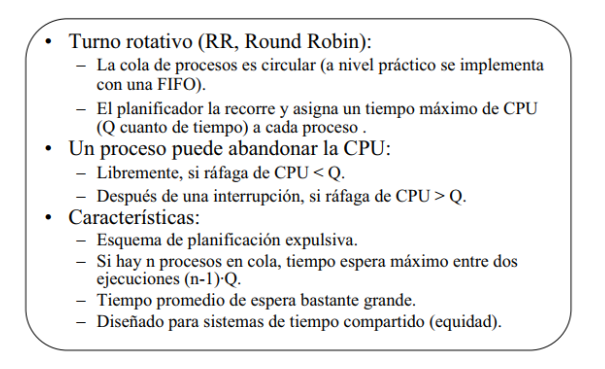
\includegraphics[width=0.55\linewidth]{rr.png}
      \caption{Funcionamiento de Round Robin.}
      \label{fig:RR}
\end{figure}

Los conceptos a tener en cuenta en el algoritmo de este metodo son:
\begin{enumerate}
    \item \textbf{Quantum}: Numero maximo de intervalos de tiempo que un proceso puede usar la CPU.
    \item \textbf{Tiempo de llegada}: Intervalo de tiempo en que comienza el proceso.
    \item \textbf{Tiempo de ejecucion o Rafaga}: Intervalo de tiempo que demora un proceso en ejecutarse.
    \item \textbf{Tiempo de finalizacion}: Intervalo de tiempo en que termina el proceso.
    \item \textbf{Tiempo de retorno}: Suma de intervalos que mide desde que comienza el proceso hasta que finaliza su ejecucion.
\end{enumerate}

\subsection{Tablas Hash}
Otro proposicion que podriamos hacer, pero no asegurar es la utilizacion de tablas hash, la cual es un contenedor asociativo que permite el almacenamiento de entradas con una clave unica para luego ser recuperadas posteriormente de manera eficiente, debido a que la clave es unica para cada entrada entonces se puede usar a esta clave como un identificador.

Su estructura hace que la recuperacion de informacion sea eficiente con un tiempo constante, sin embargo, esta tabla hash frecuentemente se producen colisiones, esto se pasa generalmente cuando una clave se genera para dos entradas, sin embargo esto tiene solucion gracias a que ya cuenta con una funcion de resoluciones de colisiones, por eso existen dos tipos de tablas hash en funcion a como se resulven sus colisiones:

\begin{itemize}
    \item Encadenamiento separado: Las colisiones se resuelven insertandolas en una lista.
    \item Direccionamiento abierto: Se usa un vector como representacion y cuando ocurre la colision, le volvemos a reasignar otra clave no repetida.
\end{itemize}

\begin{figure}[thpb]
    \centering
    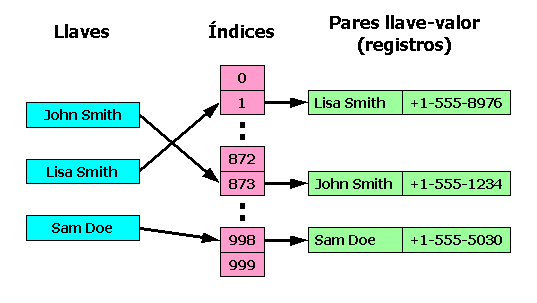
\includegraphics[width=0.55\linewidth]{Tabla_hash1.png}
    \caption{Caption}
    \label{fig:hash}
\end{figure}

Las operaciones que se pueden utilizar en una tabla hash son:
\begin{itemize}
    \item Insertar: Puede ser un valor entero o una cadena de caracteres.
    \item Borrar: Si uno quiere borrar un nodo debe seleccionar dicho nodo.
    \item Vaciado de lista: Elimina todos los elementos de la tabla
\end{itemize}

\section{Estado del Arte}
Con los dos metodos mencionados anteriormente, puede mejorarse el modelo de servidor - esclavo que se propone, veamos como el modelo Round Robin puede ayudar.

De acuerdo con algunos articulos cientificos el metodo Round Robin es utilizado en modelos de metodologia empirica, la cual propone un modelo matematico en una comparacion de un evento con su numero de participantes (ejemplo de una liga de futbol con su numero de participantes).

\begin{figure}[thpb]
    \centering
    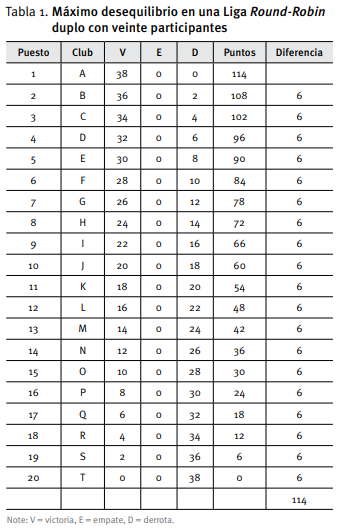
\includegraphics[width=0.55\linewidth]{tabla.png}
    \caption{Resultados de un metodo doble Round Robin}
    \label{fig:tabla}
\end{figure}

Considerando el ejemplo anterior donde se utiliza el metodo doble Round Robin, el analisis de este ejemplo considera que en todo torneo o liga hay un porcentaje de desequilibrio en el balance competitivo. Algunos investigadores destacan la posibilidad de utilizar metodos estadisticas para buscar diferencias significativas entre las medias de los distintos torneos.

\section{Metodologia o diseño del proyecto}
El proyecto consiste en la distribucion de cargas a traves de un proceso Servidor (maestro) y los otros procesos seran aquellos que  trabajen las cargas (esclavos), para plasmar esta idea en codigo se propone hacerlo en lenguaje java donde se compondra de dos partes:

\begin{itemize}
    \item \textbf{Servidor}: Se encargara de la distribucion de tareas o cargas, ademas vera que los todos los procesos esten ejecutando correctamente.
    \item \textbf{Cliente}: Se encargara de la ejecucion de las tareas que se den y una vez resuelta esta devolvera al servidor.
\end{itemize}


\section{Conclusiones}
Se propuso la estructura y forma del proyecto, los cuales estaran en constantes pruebas para obtener una buena distribucion de cargas.\\

Se propuso los metodos de Round Robin y Tabla Hash para que los procesos puedan tener una mejor eficiencia en la distribucion y ejecucion de tareas.\\

Se mostro un modelo ejemplo de como se puede utilizar el metodo Round Robin para un caso real con probabilidades.

\begin{thebibliography}{1}
\normalsize
\bibitem{}
Franck, E. (2014), \emph{Financial fair play in European football clubs: What is it all about? International Journal of Sports Finance, 9(3), 193-217.}
\\
\bibitem{}
Haan, M., Koning, R. H., & Witteloostuijn, A. (2007), \emph{Competitive balance in national European soccer competitions. In J. Albert, & R. H. Koning (Eds.). Statistical thinking in sports (Chap. 4, pp. 63-76). London: Taylor and Francis.}
\\
\bibitem{}
Levin, R., Mitchell, G., Volcker, P., & Will, G. (2000), \emph{The report of the independent members of the Comissioner’s Blue Ribbon Panel on baseball economics},\\ Recuperado en: 
\url{http://www.mlb.com/mlb/downloads/blue\_ribbon.pdf}
\\
\bibitem{}
Zhiwen Chen, \emph{ student at the College of Computer Science and Electronic Engineering, Hunan University, China. His research interests are in parallel computing and multi-core systems.} 
\\
\bibitem{}
Jianhua Sun, \emph{Associate Professor at the College of Computer Science and Electronic Engineering, Hunan University, China. She received the Ph.D. degree in Computer Science from Huazhong University of Science and Technology, China in 2005. Her research interests are in security and operating systems. She has published more than 70 papers in journals and conferences, such as IEEE Transactions on Parallel and Distributed Systems}, IEEE Transactions on Computers.
\\
\bibitem{}
Víctor M. Alfaro Ruíz, \emph{Métodos de sintonización de controladores PID que operan como reguladores}, San José, Costa Rica, 2002.\\ Disponible en: 
\url{http://eie.ucr.ac.cr/uploads/file/documentos/pub_inv/articulos/valfaro02B.pdf}

\end{thebibliography}
\end{document}